\section{Dataset Description}
\label{sec:dataset_description}
In Chapter \ref{chapter:research_plan}, we have outlined our primary research focus, which revolves around the field of Multi-Task Imitation Learning. Specifically, we are directing our attention to methods based on video conditioning, with reference to seminal works such as \cite{mandi2022towards_more_generalizable_one_shot} and \cite{dasari2021transformers_one_shot}, which have been chosen as our initial reference points due to their promising outcomes, as presented in Table \ref{table:mosaic}.
In this context, we aim to establish a robust baseline for tasks that encompass a blend of highly multimodal behaviors and fine-grained manipulations. To achieve this, we have commenced our investigations by narrowing our focus to two specific tasks: \textit{``Pick-and-Place"} and \textit{``Nut-Assembly"} both of which are proposed among the seven tasks in \cite{mandi2022towards_more_generalizable_one_shot}.
\paragraph{Simulated Dataset} \mbox{} \\
Table \ref{table:reference_dataset_cardinality} provides a summary of the dataset's cardinality, including the number of variations for each task and the number of trajectories collected for each variation. These statistics align closely with the parameters outlined in \cite{mandi2022towards_more_generalizable_one_shot}.
\begin{table}[htb]
    \centering
    \caption{Reference dataset's cardinality}
    \label{table:reference_dataset_cardinality}
    \begin{tblr}{
        width = \linewidth,
        colspec = {Q[192]Q[165]Q[387]Q[190]},
        cells = {c},
        hlines,
        hline{1,4} = {-}{0.08em},
            }
                              & \textbf{\#Variations} & \textbf{\#Trajectories per variations} & \textbf{\#Trajectories} \\
        \textit{Pick-Place}   & 16                    & 100                                    & 1600                    \\
        \textit{Nut-Assembly} & 9                     & 100                                    & 900
    \end{tblr}
\end{table}

In the simulated environment, agent trajectories $\tau^{j}_{m_{i}} = \left \{ s_{0}, a_{0}, s_{1},\dots, a_{T-1}, s_{T}\right \}$ are generated using predefined manual control strategies. The robot's actions are determined by programs that rely on accurate information provided by the environment, such as the target object and the desired placement location. During trajectory execution, various elements are recorded, including a frontal view image of the scene (see Figure \ref{fig:first_variation}) to represent the state $s_{t}$ and the robot's gripper pose to represent the action $a_{t}$. In addition to agent trajectories, we have also collected demonstrator examples under the same scenarios and cardinality as detailed in Table \ref{table:reference_dataset_cardinality}. However, in this case, we changed the robot from the Universal Robot UR5e to the Franka-Emika Panda. For the demonstrator, we are specifically interested in recording only frontal view images of the scene, as we use the execution video of command $c_{m_{i}}$. Figure \ref{fig:example_of_variations_for_pick_place} and Figure \ref{fig:examples_of_variations_for_nut_assembly} illustrate some examples of variations for each task
As it can be noted the designed scenarios show some difficulties:
\begin{itemize*}[label=$(\bullet)$]
    \item In the dataset a given object (e.g., the red box) plays the role of both target object and distractor. This poses a significant challenge because the method cannot learn a pre-established pattern where a specific category of objects consistently assumes the role of the target while another category consistently acts as a distractor. Consequently, the demonstration video and its role in conditioning the policy become pivotal factors in addressing this challenge;
    \item The objects in a given task share the same category and the same shape (e.g., in pick-place there are only box with the same dimensions). This characteristic can increase the complexity in target object localization task because methods need to acquire high-level features, such as color, to distinguish between different objects in the scene.
\end{itemize*}

\noindent As discussed in Section \ref{sec:research_activity}, these factors play a pivotal role and can significantly impact the performance of the methods employed.
Another critical consideration pertaining to the dataset concerns the distribution of actions. This aspect is exemplified in Figure \ref{fig:dataset_distribution}, which illustrates the trajectory distribution along the y-axis, that is parallel to the table and most involved during task execution. It is evident that, for a given variation, the target object exhibits varying starting positions. This characteristic adds a layer of complexity to the learning task because the model must generalize to different starting position of the target object.
\begin{figure}[hbt!]
    \centering
    \begin{subfigure}{0.2\textwidth}
        \centering
        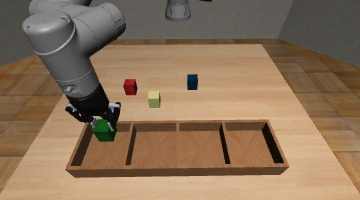
\includegraphics[width=\textwidth]{Figures/images/pick_place/task_1.png}
        \caption{First variation, green box into first bin}
        \label{fig:first_variation}
    \end{subfigure}
    \hfill
    \begin{subfigure}{0.2\textwidth}
        \centering
        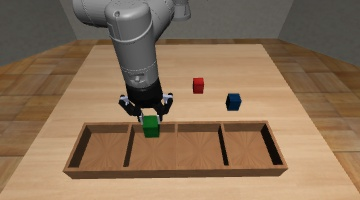
\includegraphics[width=\textwidth]{Figures/images/pick_place/task_2.png}
        \caption{Second variation, green box into second bin}
        \label{fig:second_variation}
    \end{subfigure}
    \hfill
    \begin{subfigure}{0.2\textwidth}
        \centering
        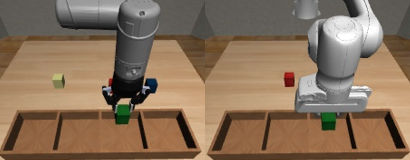
\includegraphics[width=\textwidth]{Figures/images/pick_place/task_3.png}
        \caption{Third variation, green box into third bin}
        \label{fig:third_variation}
    \end{subfigure}
    \hfill
    \begin{subfigure}{0.2\textwidth}
        \centering
        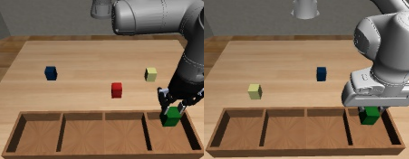
\includegraphics[width=\textwidth]{Figures/images/pick_place/task_4.png}
        \caption{Fourth variation, green box into fourth bin}
        \label{fig:fourth_variation}
    \end{subfigure}
    \caption{Example of variations for the Pick and Place task. The same set of variations is repeated for each block}
    \label{fig:example_of_variations_for_pick_place}
\end{figure}

\begin{figure}[hbt!]
    \centering
    \begin{subfigure}{0.2\textwidth}
        \centering
        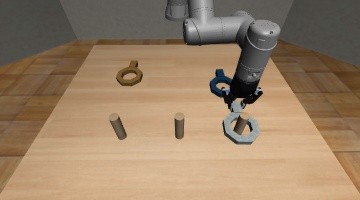
\includegraphics[width=\textwidth]{Figures/images/nut_assembly/task_1.png}
        \caption{First variation, assembly gray nut with right peg}
        \label{fig:first_variation_nut}
    \end{subfigure}
    \hspace{30px}
    \begin{subfigure}{0.2\textwidth}
        \centering
        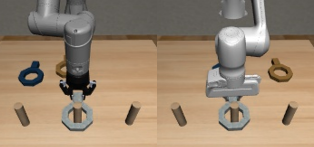
\includegraphics[width=\textwidth]{Figures/images/nut_assembly/task_2.png}
        \caption{Second variation, assembly gray nut with middle peg}
        \label{fig:second_variation_nut}
    \end{subfigure}
    \hspace{30px}
    \begin{subfigure}{0.2\textwidth}
        \centering
        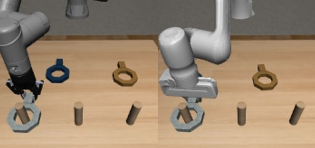
\includegraphics[width=\textwidth]{Figures/images/nut_assembly/task_3.png}
        \caption{Third variation, assembly gray nut with left peg}
        \label{fig:third_variation_nut}
    \end{subfigure}
    \caption{Example of variations for the Nut-Assembly. The same set of variations is repeated for each nut}
    \label{fig:examples_of_variations_for_nut_assembly}
\end{figure}
\begin{figure}[htb]
    \centering
    \begin{subfigure}[b]{0.9\textwidth}
        \centering
        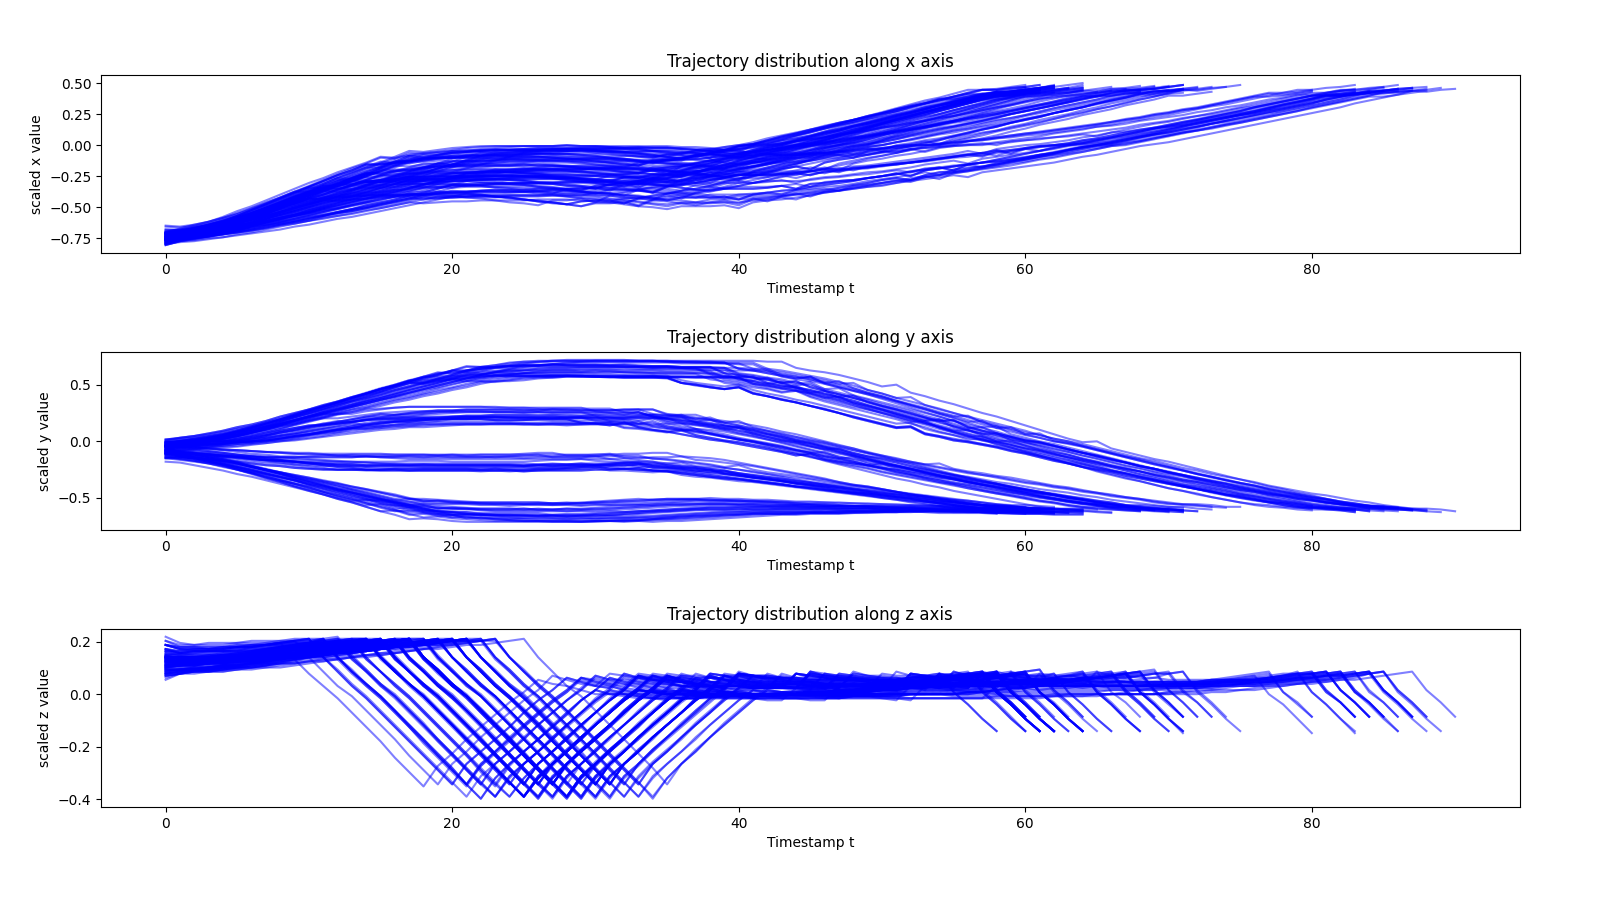
\includegraphics[width=\textwidth]{Figures/images/dataset_distribution/pick_place_variation_0.png}
        \caption{Trajectory distribution along the x-y-z axes for the first Pick-Place variation}
        \label{fig:pick_place_first_variation}
    \end{subfigure}
    \hfil
    \begin{subfigure}[b]{0.9\textwidth}
        \centering
        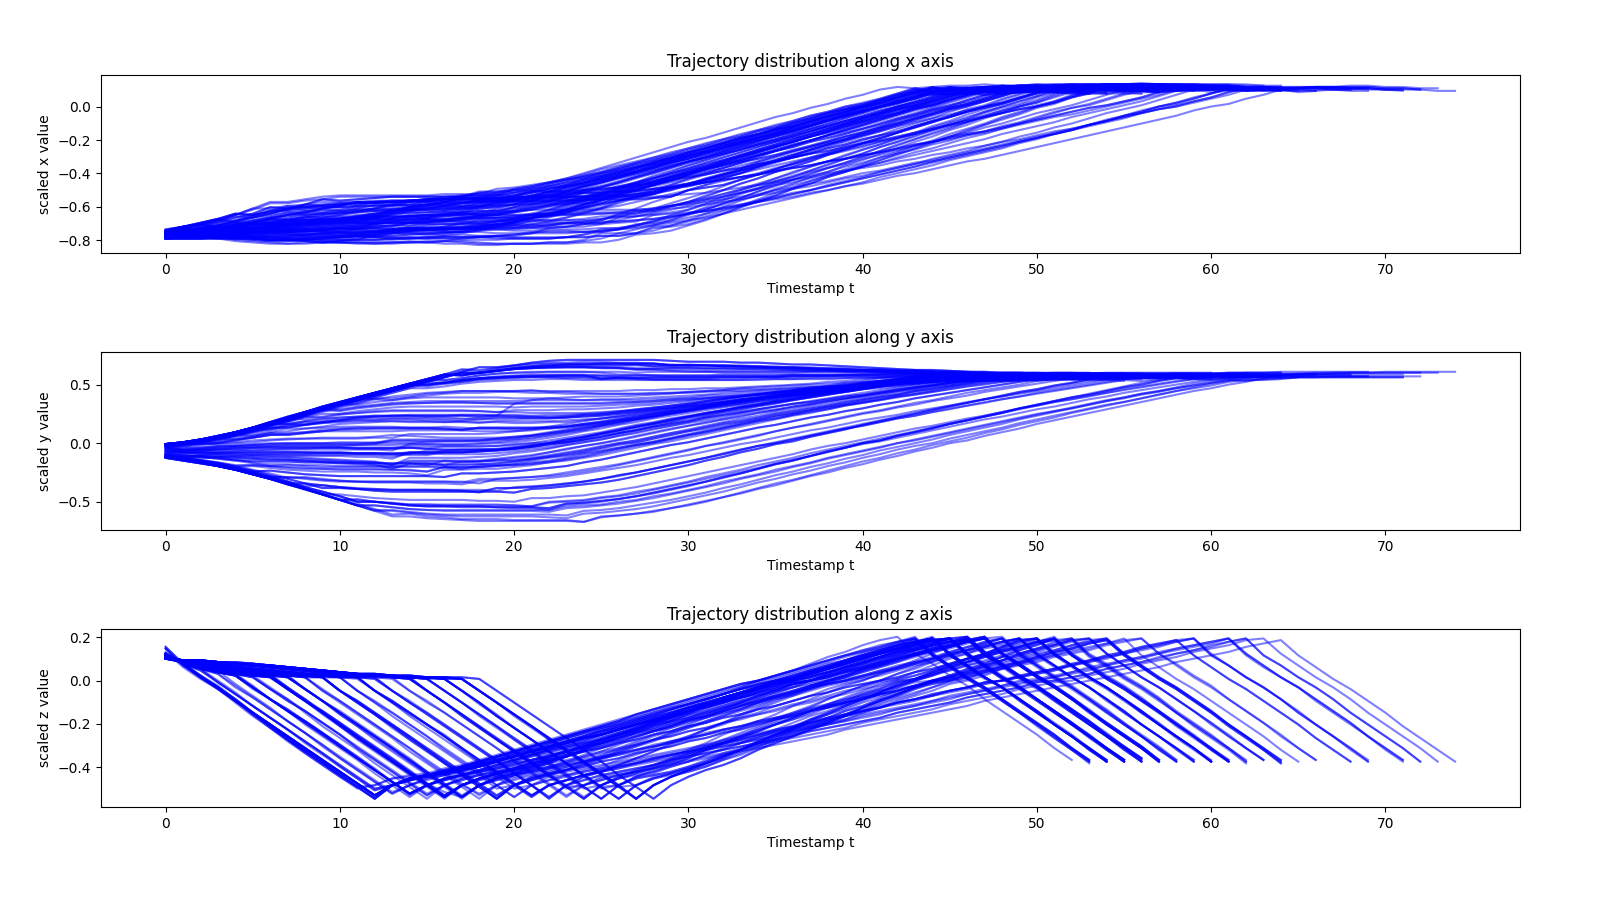
\includegraphics[width=\textwidth]{Figures/images/dataset_distribution/nut_assembly_variation_0.png}
        \caption{Trajectory distribution along the x-y-z axes for the first Nut-Assembly variation}
        \label{fig:nut_assembly_first_variation}
    \end{subfigure}
    \caption{Trajectory Distribution along the x-y-z axes for the first variation of Pick-Place (\ref{fig:pick_place_first_variation}) and Nut-Assembly (\ref{fig:nut_assembly_first_variation}) task}
    \label{fig:dataset_distribution}
\end{figure}


\textbf{Real-World Dataset and Setup}  \mbox{} \\
During this second year we also designed and implemented an experimental setup in a controlled environment that allows the evaluation of the proposed methods on a real robotic platform. It is composed of:
\begin{itemize*}[label=$(\bullet)$]
    \item The UR5e robot \cite{ur5e}, endowed with the Robotiq2f-85 gripper \cite{robotiq}, that will play the role of the agent;
    \item 4 Zed-Mini stereo cameras \cite{zed}, 1 camera is mounted on the gripper while the other three are mounted around the robot in order to have complete coverage of the workspace.
\end{itemize*}
Also in real-world setup we consider the pick-place and the nut-assembly problem. In this case agent trajectories are obtained by \textit{teleoperating} the robot, and a dataset with the same cardinality as in Table \ref{table:reference_dataset_cardinality} is under collection. Example of pick-and-place demonstration is reported in Figure \ref{fig:real_dataset}.
\begin{figure}[htb]
    \centering
    \begin{subfigure}[b]{0.45\textwidth}
        \centering
        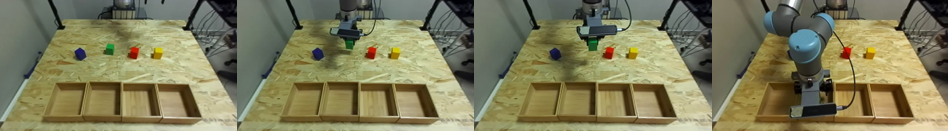
\includegraphics[width=\textwidth]{Figures/images/dataset_real_robot/frontal_camera.png}
        \caption{Frames of pick-place task from frontal camera}
        \label{fig:frontal_camera}
    \end{subfigure}
    \hspace{5px}
    \begin{subfigure}[b]{0.45\textwidth}
        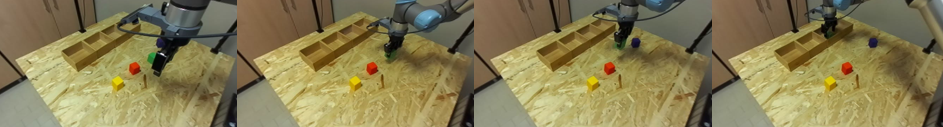
\includegraphics[width=\textwidth]{Figures/images/dataset_real_robot/lateral_left.png}
        \caption{Frames of pick-place task from lateral left camera}
        \label{fig:lateral_left}
    \end{subfigure}
    \vfill
    \begin{subfigure}[b]{0.45\textwidth}
        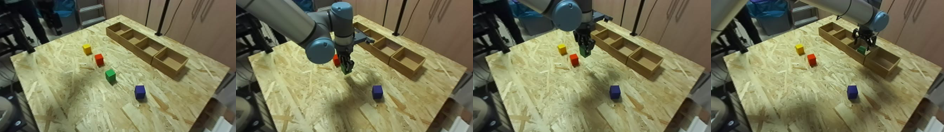
\includegraphics[width=\textwidth]{Figures/images/dataset_real_robot/lateral_right.png}
        \caption{Frames of pick-place task from lateral right camera}
        \label{fig:lateral_right}
    \end{subfigure}
    \hspace{5px}
    \begin{subfigure}[b]{0.45\textwidth}
        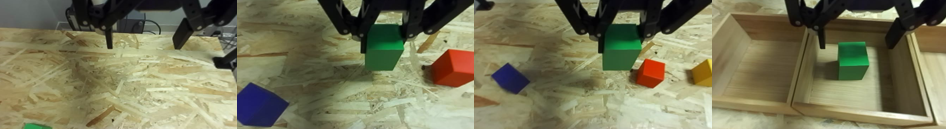
\includegraphics[width=\textwidth]{Figures/images/dataset_real_robot/gripper_camera.png}
        \caption{Frames of pick-place task from gripper camera}
        \label{fig:gripper_camera}
    \end{subfigure}
    \caption{Frames of pick-place task from different cameras}
    \label{fig:real_dataset}
\end{figure}

